% CREATED BY DAVID FRISK, 2018
\chapter{Theory}

This chapter gives a detailed description of the theoretical concepts used to support the thesis work. The chapter begins with a brief description about Balanced Scorecard framework on which most of firms base their performance measurement. Then the theory about various aspects of KPIs such as principles, characteristics, frameworks and categorization are detailed.  Thereafter, the four important support factors for KPIs are discussed one by one. In the penultimate subchapter,  the theory related to conducting and analysing interviews is presented. The final part concerns the theory related to administering and investigating the survey.

%In the following sections, examples of a figure, an equation, a table, a chemical structure, a list, a listing and a to-do note are shown.

%\section{Figure}
%\begin{figure}[H]
%\centering
%\includegraphics[width=0.45\linewidth, trim=3cm 11cm 3cm 11cm]{figure/X.pdf}
%\includegraphics[width=0.45\linewidth, trim=3cm 11cm 3cm 11cm]{figure/Y.pdf}
%\caption{Surface and contour plots showing the two dimensional function %$z(x,y)=\sin(x+y)\cos(2x)$.}
%\end{figure}

%\section{Equation}
%\begin{equation}
%f(t)=\left\{ \begin{array}{ll}
%1,~~~~ & t< 1 \\
%t^2 & t\geq 1
%\end{array}\right.
%\end{equation}

%\section{Table}
%\begin{table}[H]
%\centering
%\caption{Values of $f(t)$ for $t=0,1,\dots 5$.}
%\begin{tabular}{l|llllll} \hline\hline
%$t$ & 0 & 1 & 2 & 3 & 4 & 5 \\ \hline
%$f(t)$ & 1 & 1 & 4 & 9 & 16 & 25 \\ \hline\hline
%\end{tabular}
%\end{table}

%\section{Chemical structure}
%\begin{center}
%\chemfig{X*5(-E-T-A-L-)}
%\end{center}

%\section{List}
%\begin{enumerate}
%  \item The first item
%  \begin{enumerate}
%    \item Nested item 1
%    \item Nested item 2
%  \end{enumerate}
%  \item The second item
%  \item The third item 
%  \item \dots
%\end{enumerate}

%\section{Source code listing}
%\lstset{language=Matlab}
%\begin{lstlisting}[frame=single]
%% Generate x- and y-nodes
%x=linspace(0,1); y=linspace(0,1);

% Calculate z=f(x,y)
%for i=1:length(x)
% for j=1:length(y)
%  z(i,j)=x(i)+2*y(j);
% end
%end
%\end{lstlisting}

\section{Balanced scorecard}
%The \texttt{todo} package enables to-do notes to be added in the page margin. This can be a very convenient way of making notes in the document during the process of writing. All notes can be hidden by using the option \emph{disable} when loading the package in the settings. \todo{Example of a to-do note.}
Performance measurement has been followed in the industries since old times. As the years passed the systems used to measure performance developed adapting to the requirements. Bourne et.al (2000) mention the criticisms made on the traditional measurement systems, such as short termism, lack of strategic connection, lack of continuous improvement etc. In order to overcome them and reconsider the methods of measuring performance, different authors have come up with different frameworks to encourage a balanced view. \\ 

Kennerley et al.(2003) mention that organizations have redesigned their current management systems  to ensure that they reflect their current environment and strategies. One of the best known frameworks for multidimensional performance measurement was the Balanced Scorecard framework. It is aimed at being more proactive and emphasized on balancing financial, internal, nonfinancial and external measures. This framework has been explained in the next section. \\ 

Kaplan(1992) explains the Balanced Scorecard framework in detail, he mentions that it gives managers a way to look at the business from 4 different perspectives as mentioned above. It answers the following questions:\\

\begin{itemize}
    \item How do the customer see us?
    \item What must we excel at ?
    \item Can we continue to improve and create value?
    \item How do we look to our shareholder?\\
\end{itemize} 

\begin{figure}[H]
    \centering
    \captionsetup{justification=centering, margin=2cm}
    \vspace{1cm}
    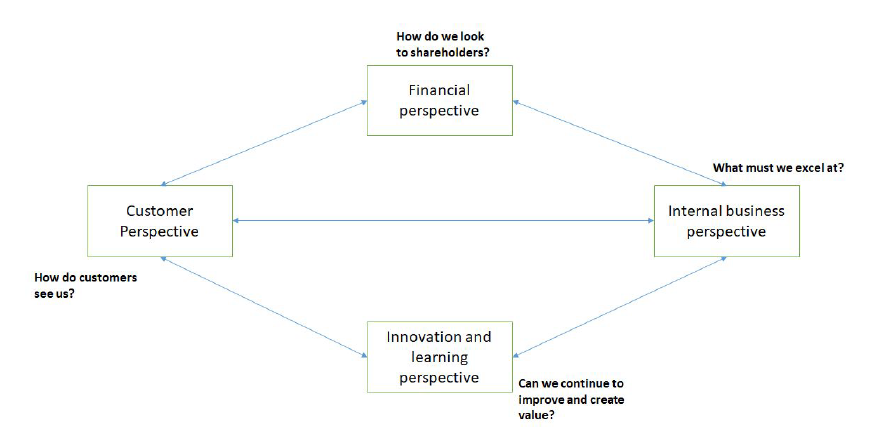
\includegraphics[width=14cm, height=9cm]{figure/auxiliary/fig41.PNG}
    \caption{Adapted from Kaplan(1992), The balanced scorecard links Performance measures}
    \label{fig:4.1}
\end{figure}


In the article they represent this framework in figure \ref{fig:4.1}:\\

\begin{enumerate}
  \item \textbf{Customer Perspective:}
            Customer is the focus for every organization. Kaplan(1992) quotes that “To be number one in delivering value to customers is a typical mission statement” making it one of the top priorities for the top management. This dimension gives the company a view on how they satisfy their customers. Are they performing well enough to deliver their best. This framework demands the managers to translate their mission statement with respect to the customer into specific targets. He mentions the 4 categories in which a customer’s concern would fall. They are time, quality, performance and service, cost. These 4 categories have been explained below:\\
  \begin{enumerate}
    \item \textbf{Time:}
    Customers value the lead time, which the time companies take to meet the needs of their customers. Depending on the situation the definition of the lead time is adapted. Kaplan (1992) exemplifies a few like, in manufacturing the products lead time is measured from the time the order is received until the product is delivered to the customer, whereas for new products the lead time is the time to market. Thus, time plays a major role in keeping the customers happy.\\
    \item \textbf{Quality:}
    It is nothing but the defect level of the products delivered to customers.\\
    \item \textbf{Performance:}
    The combination of the performance and service, measuring how the products contribute value to the customers.\\
    \item \textbf{Costs:}
    Customers see price as one single component of cost they need to pay for while dealing with the supplier. Hence, the companies need to be sensitive to balancing the costs, various costs incurred like ordering cost, scrap cost etc need to be considered to reduce the non value added costs and hence making better profits.\\
    These categories explain what factors need to be considered from a customer point of view while developing measures in the balanced scorecard.\\
  \end{enumerate}
  \item \textbf{Internal business Perspective:}
  After having the customers perspectives the managers need to focus on the factors or operations that are critical to enable them to satisfy their customers. This could be done by starting off with the factors that affect the cycle time, employee skills, productivity etc which in-turn have an impact on the customers. The top management need to consider the competencies of the employees and have a judgement on key internal processes since most of the work that affects the critical factors like cycle time, happen on workstation level or team level. This framework lets the managers make targets which in turn ensures that the team members on lower levels have clear goals or action plans that contribute to the overall mission of the company\\
  \item \textbf{Innovation and Learning perspective:}
  In the competitive environment the companies need to improvise on their existing products or services, which in turn affects the existing products and processes which make them capable to introduce entirely new products. Kaplan(1992) quotes that “ A company’s ability to innovate, improve and learn ties directly to the company’s value”. Hence, it is critical to consider and measure aspects like knowledge management, which keeps track of the innovation and learning in hand with the three other perspectives of the balanced scorecard \\
  \item \textbf{Financial Perspective:}
  Kaplan(1992) quotes that “The disparity between the improved operational performance and disappointing financial measures creates frustration in top management”. Though the market is developed and the financial measures no more lead to customer satisfaction, it is still necessary to keep track of the cash flows. He explains that the financial performance is an action of operational improvements. Apart from having the other three perspectives in the balanced scorecard, if the managers fail to convert their operational performance to the financial performance they need to rethink the strategy and implementation plans. Thus, it is necessary to directly or indirectly have financial measures in place to complete the balance scorecard.\\
\end{enumerate}

\section{KPI characteristics}
Key Performance Indicators (KPIs) defined as the navigation instruments by Marr (2019) says that they are used by the managers to keep track of the business and know if it is on a successful voyage or veering off. Parmenter (2015) defines them as the indicators that focus on aspects of organizational performance that are critical for current and future success of the organization. Due to the dynamic environment, competition satisfying the needs of customers with a certain budget is not an easy task, hence Locke and Latham (2002) say that goal setting and feedback improve productivity.\\

They are not just followed by the managers, but they act as good compass for the teams says Petaschnick (2017).  It gives them a way to visualize if they are on the right path towards the strategic goals of the organization. Zhang et al.(2017) allude that using KPIs have proved to improve quality and detect process faults and are closely related to measurable process variable which might be difficult. Choosing the right set of KPIs is challenging for the organization.\\

\subsection{General principles}
A certain set of general principles or guidelines have been put forward by Kerzner(2013) which are mentioned below:\\

\begin{itemize}
    \item KPIs are agreed to beforehand and reflect the critical success factors on the project. 
    \item KPIs indicate how much progress has been made toward the achievement of the project’s targets, goals, and objectives. 
    \item KPIs are not performance targets. 
    \item The ultimate purposes of a KPI are the measurement of items directly relevant to performance and the provision of information on controllable factors appropriate for decision making that will lead to positive outcomes. 
    \item Good KPIs drive change but do not prescribe a course of action. They indicate how close you are to a target but do not tell you what must be done to correct deviations from the target. 
    \item KPIs assist in the establishment of objectives to be targeted with the ultimate purpose of either adding value to the project or achieving the prescribed value. 
    \item KPIs force us to look at the future, whereas metrics alone may allow us to get bogged down looking at history. \\ 
\end{itemize}


\subsection{Characteristics}
 The characteristics of good KPIs have been described by various authors in different ways. Though they have a similar basic concept, the characteristics might vary. Based on the literature study conducted, Kerzner(2013) mentions 12 characteristics of a good KPI. This list of characteristics covers most of them and thus have been described  below:\\
 
 
 \begin{itemize}
     \item \textbf{Aligned:}
     The KPIs need to be linked or must be in line with the corporate strategy of the company.\\
     \item \textbf{Owned:}
     They need to be owned by an individual or a group of people. This makes someone accountable to collect the data, analyze and keep track of that KPI.\\
     \item \textbf{Predictive:}
     This basically means the KPIs need to be leading in nature. The KPIs measure drivers of business value.\\ 
     \item \textbf{Actionable:}
     The KPIs need to be timely and with actionable data, which helps the users of those KPIs can intervene to improve the performance before it is too late.\\ 
     \item \textbf{Few in Number:}
     The KPIs need to focus on a very few high valued tasks, which means they must not scatter their attention on other tasks. \\
     \item \textbf{Easy to understand:}
     The KPIs should be clear and straightforward to understand. It must be easy for the influencers to easily judge on how they can impact the results and take necessary actions to perform better.\\
     \item \textbf{Balanced and linked:}
     The KPIs need to reinforce each other and not suboptimize each other.\\
     \item \textbf{Trigger changes:}
     Continuous improvement is one of the key for success, measuring these KPIs should trigger positive changes in the organizations.\\ 
     \item \textbf{Standardized:}
     It means that the KPIs must have a defined set of rules and standard definitions. Across the cross functional teams they need to have similar calculation and standard way to conclude the results.\\ 
     \item \textbf{Context driven:}
     KPIs put the performance in certain context by the use of targets so the users can gauge their progress over time.\\ 
     \item \textbf{Reinforced with incentives:}
     The impact of the KPIs can be magnified by attaching incentives to them. This keeps the employees motivated and follow the KPIs.\\ 
     \item \textbf{Relevant:}
     KPIs eventually loose their impact over time. As the time proceeds they need to reconsidered and refreshed periodically.\\

 \end{itemize}

Apart from these characteristics, frameworks were proposed by authors to set goals and KPIs. One such framework is SMART, which has been described in the next section. \\

\subsection{SMART framework}
“The establishment of objectives and the development of their respective action plans are the most critical steps in a company's management process,” says Doran(1981). It is clear that objectives or goals are different from the action plans, and these actions plans act as the indicators to measure if the organization is moving towards the right goals. Shahin(2006) also gives examples of how the key performance indicators are different from the actual goals of the organization. He mentions that the indicators are used to measure the progress towards achieving the goals, and each of them must be based on criteria that make them easy for analysis. Most often used model which describes these criteria is the SMART( Specific, Measurable, Attainable, Realistic and  Time Sensitive), which is represented in figure \ref{fig:4.2}.

\begin{figure}[H]
    \centering
    \captionsetup{justification=centering, margin=2cm}
    \vspace{1cm}
    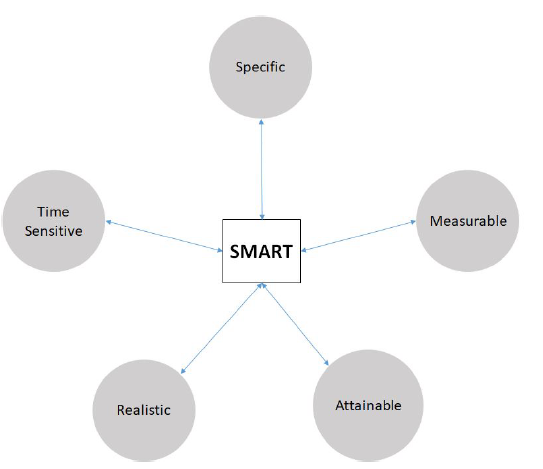
\includegraphics[width=10cm, height=9cm]{figure/auxiliary/fig42.PNG}
    \caption{Adapted from Shahin(2006), SMART Model}
    \label{fig:4.2}
\end{figure}

Each of these criteria have been explained below:

\begin{itemize}
    \item \textbf{Specific:}
    The measures need to be as distinct as possible and detailed enough. If the measures are broad and not desirable, it is difficult to analyze the root causes in case they are not met. \\

    \item \textbf{Measurable:}
    The KPIs need to be easily measurable and an indicator of progress, it is a way to ensure that the goal has been achieved or not. They could be qualitative or quantitative, but not ambiguous. It also helps to base decisions on facts which are measured, clear and concrete. To do so, the measures need to be tallied against a certain standard of performance or expectation.\\

    \item \textbf{Attainable:} The set of measures should not be out of reach. They need to be practical, based on the resources and potential to achieve the targets.  \\
  
    \item \textbf{Realistic:}
    Extending the concept of being attainable, they need to be realistic for the given working conditions. As Shahin (2016) quotes that “Being realistic in the choice of goals in helpful in examining the availability of resources and selecting KPIs..\\

    \item \textbf{Time sensitive:} For every measure there needs to be a certain time frame in which it needs to be successfully achieved. It is helpful to breakdown and plan the indicators or tasks and measure success along the path of reaching that particular goal. Toledo(2005) says that this assists in developing a realistic action plan.  \\

\end{itemize}

Apart from these definitions of the SMART goals setting, a new acronym SMARTER has also been developed as described by Wade(2009). In this framework E represented evolving and R represented Recorded or reviewed which are described below:\\

\begin{itemize}
    \item \textbf{Evolving:}
    Hersh(2012) mentions that the measures change with time. As the time progresses, the resources and capabilities change, the goals also must be re-tuned or reconsidered.\\   

    \item \textbf{Recorded:}
    The measures need to be documented and updated from time to time\\
\end{itemize}

This framework was described differently in the distinct articles. Each letter was slightly adapted to the situations described in those papers. Hence, they were collected and adapted from Wade (2009) as follows\\

S- Specific, significant, stretching, simple, stimulating, straight forward, self owned, self managed, self controlled, strategic
M- Measurable, meaningful, motivational, manageable, maintainable 
A- Attainable, agreed upon, actionable, ambitious, acceptable, aligned, accountable, achievable
R- Realistic, relevant, reasonable, rewarding, robust reviewable
T- Time sensitive, tangible, trackable, tactical, traceable
E-Ethical, exciting, enjoyable, evaluated, engaging
R- Recorded, reviewed, rewarded, resourced, research based etc.

\subsection{Categorizing KPIs}
Smith R(2001) defines KPIs as the indicators that combine several metrics to yield objective performance facts. Two such metrics are:\\

\begin{itemize}
    \item Financial and non-financial KPIs
    \item Leading and Lagging Indicators \\
\end{itemize}
Such categorization is done based on what the KPIs intend to indicate. These have been explained in the section below:\\

\subsubsection{Financial and Non-Financial KPIs}
White(1996) mentions that historically the way used to measure a company`s performance have been the financial measures. The indicators that represent the financial values are categorized as the financial KPIs. Kaplan(1992) describes the typical financial goals as the ones which have to do more with the profitability, growth and shareholder value. Parmenter (2009) in his book suggested cost of goods sold / sales, scrap cost as \% age of total sales, A/c Receivable turnover, cash flows, days in inventory, days sales in receivables, net income, sales, number of profitable customers, return on equity, sales by product, sales growth rate, return on assets and return on capital employed as the measures of the financial performance of the organizations. Bhatti et al.(2014) also describes about the use of financial KPIs to measure the performance. \\
The other category of non-financial indicators are the ones which focus on other aspects for instance cycle time, customer satisfaction etc.\\ 

\subsubsection{Leading and Lagging Indicators}

Another set of a category that could be used is based on the values of them the KPIs, they can be classified into two different categories, leading and lagging indicators. Smith R(2001) explains the two categories with a live example. He gives an example of a person driving a car down a road. When a driver deviates from the driving lane and veers on the shoulder of the road the tires run over “out of lane” indicators. He correlates these lanes to KPIs which are approaching a critical condition. Such are the leading indicators which measure and track performance before problems arise.  \\

In the same driving situation, in case there was no “out of lane” indicator the car would go offroad when a reactive approach would be needed to fix issues. This is correlated to a lagging indicator where the problem can be approached of solved only after damage has been caused. Based on this understanding the two categories have been elaborated below:\\

\begin{itemize}
    \item \textbf{Lagging indicator:}
    These are the indicators which depict measured which could be used to analyze only after the results are obtained. Manuele(2009) mentions that it is defined as a measure that only changes after the changes are done and such indicators are helpful in confirming the trends. Mannick et al. (2019) name them as the “after-the-fact” indicators, measuring the events that have already happened. He states that they are reactive in nature, since the data from the past periods could be used for future developments and organizational responses often occur in reaction to such measurements\\  

    \item \textbf{Leading indicator:}
    The indicators under this category are the ones which present or depict a trend which could be used to predict the future. Manuele(2009) describes them as it is a measurable factor that changes before the results follow a  particular pattern or trend. The changes in these indicators may foresee the results, although not with great accuracy. These are typically input oriented indicators which concern with the efficiency of analyzing if the work is done in the right direction.\\
\end{itemize}


\section{Support factors for KPI´s}
Choosing the right KPIs is a very important aspect to drive the business, apart from that it is also important to ensure few soft aspects which trigger the successful implementation of those KPIs. Kerzner(2013) in his book states several reasons for failure of KPIs like people believing it was the task of line managers, employees believing that their actions do not contribute to the KPIs etc. This proves that these soft aspects need to be taken care of while implementing the KPIs. Few of them used in this thesis work have been elaborated below.\\

\subsection{Top management interest/vigour}
Cox et al.(2003) proves in his research that based on the level of experience and position of the stakeholders in an organization, the level of interest and involvement for using the KPIs varies. Young et al.(2008) assert that ‘when a senior management project sponsor/champion, the CEO and other senior managers devote time to review plans, follow up on results and facilitate management problems’. They also added that the time spent must be proportional to the cost and be aware of the updates. As the teams follow their leaders, it is very important that the top management should follow the KPIs. \\

\subsection{OKR - Objective and Key Results}
The author of the book “Measure what matters” (Doerr, 2019) defines the OKR model as a collaborative goal setting protocol for companies, teams and individuals. An “Objective” is simply what is to be achieved. Nothing more or less. Therefore, they need to be concretely defined, action oriented and provide inspiration to people.\\
“Key Results” are used to monitor how the objectives are achieved. Therefore, the period should be defined, they should be aggressive in nature and feasible to achieve. The author also suggests that there should not be more than 5 objectives and each objective should have 3-5 key results associated with it.\\

Basically, OKR is a framework which provides a lot of freedom for the employees to set their targets and encourage them on specifically how they want to measure the progress. It combines responsibility and challenges which in turn makes the employees to be more organized in their goal setting. Using this method, it will be easy for top management as well to clearly measure the performance of employees.\\

The 4 OKR superpowers mentioned by Doerr (2018) are:\\

\begin{itemize}
    \item \textbf{Focus and commit to priorities:}
    OKRs push the leaders to make fixed decisions thus increasing the focus area and removing any ambiguity. Also, they act as a precise communication tool for teams and the individual employees.\\

    \item \textbf{Align and connect for teamwork:}
    With OKR transparency, the goals from CEO till Interns are available to everyone. This enables individuals to link their objectives to the top management strategy and coordinate horizontally with other team members.\\

    \item \textbf{Track for accountability:}
    As OKRs are constantly checked with the progress discussed frequently, the accountability increases as individuals measure their progress with hard data. But it is important to conduct it in no judgment accountability.\\

    \item \textbf{Stretch for amazing:}
    OKRs motivate the people to work hard and achieve their objectives by constantly monitoring their key results. It provides the freedom to fail and be creative.\\
\end{itemize}

Until now, the theory and benefits of OKR mentioned by the author is discussed. In the next part, the adaptation of OKRs by Volvo Group is presented. Volvo wishes to employ this idea of OKR in their tool to measure the performance. The tool is named as “Performance touchpoint”.\\

Here the main focus is how Volvo encourages it employees to set the goals, format for breaking down the goals and the guidelines presented. All the data is obtained from the Performance touchpoint page (2019) available from the intranet website Violin..\\

\begin{enumerate}
    \item \textbf{Setting the goals:} The three main questions to be asked here are.\\

        \begin{itemize}
            \item Where do you want to go? (The objectives)
            \item How you will know that you are getting there? (Key results)
            \item What will you do to get there? (Key actions)\\
Based on the idea behind the three questions the employees are guided to set their goals.\\
        \end{itemize}
        
    \item The breakdown of the top level objectives into daily tasks is neatly described in the figure \ref{fig:4.3}\\

    \begin{figure}[H]
    \centering
    \captionsetup{justification=centering, margin=2cm}
    \vspace{1cm}
    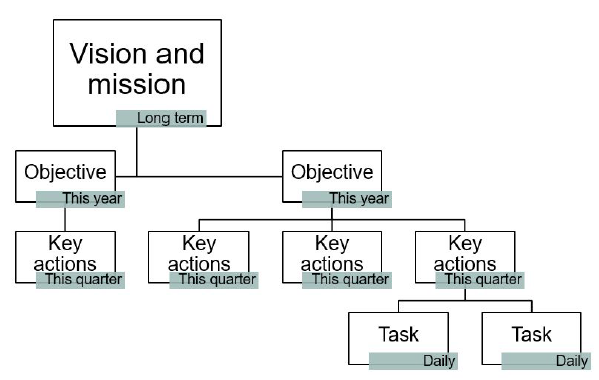
\includegraphics[width=12cm, height=7.5cm]{figure/auxiliary/fig43.PNG}
    \caption{Breakdown of the top level objectives into daily tasks}
    \label{fig:4.3}
    \end{figure}


    If all employees follow the model, their daily tasks will be automatically aligned to the vision of the company. The intervals of key actions and objectives which are refreshed quarterly and annually respectively, provide appropriate time for employees to change the focus areas and work on new found problem sector.\\

    \item \textbf{Guidelines:} Some of the guidelines to create the OKRs are:\\
    \begin{itemize}
        \item \textbf{Set them annually and quarterly:} This provides adequate time to achieve something in a business context and also feasibility to judge the achievements.\\
        \item \textbf{Do not have too many:} 5 objectives with less than 4 key results each per quarter should be the limit. This is in accordance with the suggestion given by Doerr.\\ 
        \item \textbf{Make the priorities challenging:} As the goals become more challenging, it encourages the employees to strive hard and innovate.\\
        \item \textbf{A key result must be defined:} A learning process needs to be created.\\
\end{itemize}
\end{enumerate}
Overall,the discussion above combines the descriptions about OKR from both the Original author John Doerr and the adaptations of how it will be used in Volvo.\\



\subsection{Strategy Cascading}
Initially the definition of strategic cascading is provided along with the true nature of cascading and what it should consider. Later the need for cascading is described and this section is completed with briefly presenting the benefits of strategic cascading.\\

Strategy cascading plays an important role in aligning all the engineers/employees towards the generic goal of the company. Decoene (2006) defines cascading as “The cascading process is a systematic approach to align the strategic business objectives to the operational performance measures and actions”\\



Usually, based on personal experience this cascading is considered wholly as a top management affair. But Loch (2008) argues that “the key benefit from cascading lies not in top-down control, but in clarity for the technical personnel about what they can contribute, in the motivation that stems from being able to voice their views and concerns, and in the dialogue between senior management and the R&D organization”. Employees who are not aware of the strategy will not be in a position to take better decisions which are aligned to the objectives. This in turn may reduce the motivation level and interest of employees causing them to pull the rope in the opposite direction. Therefore, establishing effective connection between the technical work of engineers and the overall business strategy is a major challenge for the top management.\\

Schlickel et. al (2013) in their research describe the need for efficient strategy cascading. After detailed research on 9 firms, they conclude that increase in the quality of strategic cascading is associated with increased performance of the firm. Therefore, focus should be given to better quality cascading of strategic goals into functional targets.\\

Benefits of strategic cascading:
Loch (2008) lists the 3 important benefits of strategic cascading.\\

\begin{itemize}
    \item \textbf{Clarity of what the organization is going to achieve:} 
    When the middle management and the end employees are clear about the organization goals designed by senior management, why they are present and what role they should play to make it possible, it creates the road for success.\\
    \item \textbf{Ability to negotiate and involvement of people in their own measure:}
    This freedom will result in efficient cross-functional activities where people come together to create own measures and negotiate the end result with the authorities.\\
    \item \textbf{Ensures fair process:} 
    Fair process refers to the observation that if decisions are made with transparency , engagement , and clarity about the effects, then people feel better about the decisions and are more motivated to comply and actively contribute (Loch, 2008).\\
\end{itemize}

Overall, it is evident from the literature that importance needs to be given to strategic cascading considering the long lasting and extended benefits from it.


\subsection{Visual Communication}
Communication is the key to success in organizations. Griffith (2002) mentions in his article that, “communication underlies the effectiveness of coordinating exchange activities, developing strong relationships which in turn results in improved performance.'' As coordination forms a major part to get alignment, much attention has to be given to communication. Kernbach (2015) also quotes that “One key for the better execution of strategies is to engage employees through a better way of communicating the strategy”. One of the effective ways is to communicate visually. Horn (1998); Huff (1990); Kosslyn (2007); Lehtonen (2011); Tversky (2004) and several authors explain how visualization is an efficient way to communicate in business. If an employee is not able to picture the progress of what is being done, the goals or objectives which are not documented and visualized, then there is a fear of employees losing focus on the targets.\\

Kernbach(2015) based on an experiment proves that visual communication of the strategic goals was very much necessary for the employees to connect to them. Toyota is a wonderful example, where Hoshin kanri boards are placed at each levels of hierarchy breaking down the goals and measuring the progress continuously. Quantitatively, Kaplan (2008) in his study proves that 73\% of the companies showed outstanding performance just by clearly communicating their strategy. Whereas only such actions were taken by only 28\% of the underperformers.
\\

\section{Theory on research methods}

This segment presents the theory behind the usage of two prominent empirical data collection methods. Namely, Interviews and Survey.

\subsection{Interviews}
The section begins with defining a qualitative interview with brief description of face to face interviews. Then various suggestions provided by academics on things to be done before, during and after the interviews are described. In the next part, the information about the thought process about interview questions is presented. The latter part of the section describes the two analysis methods used to investigate the interview data. \\

As the research was qualitative in nature, interviews were primary method to gather empirical data.  Kvale (1983, p.174) defines a qualitative research interview as "an interview, whose purpose is to gather descriptions of the life-world of the interviewee with respect to interpretation of the meaning of the described phenomena". \\ 

After consideration of the advantages and possibility, option of face to face interview was finalized. According to Opdenakker(2008) Face to Face interviews are characterised by synchronous communication in time and place. Also, in FtF interviews there is no significant time delay between question and answer; the interviewer and interviewee can directly react on what the other says or does. Thus, considering the advantages of this type of interview method, we conducted all our interviews for this research using face to face direct interviews.\\

Later, after zeroing in on face-to-face semi structured interviews to suit our study, the next step was to take the considerations to be taken during the whole interview process. The process is divided into three steps and discussed briefly.\\

\subsubsection{Before interview}
As Knox et, al (2009) describe in their article, semi structured interviews, in which a protocol using open-ended questions based on the study’s central focus is developed before data collection to obtain specific information and enable comparison across cases. This provided the interviewees to be flexible in their answers and also the possibility for the interviewers to delve more into specific. Now, as the idea behind the interview is fixed, the next part is to think about the procedures. As Scheinberg (2018) recounts in her lecture, the steps to be taken before the interview are consider what you want to observe during the interview, need to know how you will record the information and how the results are analysed with the decision to handle the data collected. This provides a clear direction for the interviewees. Along with this, the basic gesture of informing the interviewees about the intention of interviews, the date and duration of the interview was also discussed. \\

\subsubsection{During interview}
Scheinberg (2018) informs in her lecture that the following steps need to be taken during the interview.\\

\begin{itemize}
    \item State the purpose and intention of the interview clearly 
    \item Explain the background context of the questions
    \item Clearly inform what is important for you and what do you want to learn from the interview
    \item Indicate the flow of the interview
    \item Give permission for the interviewee to stop if needed
    \item Inform what will happen with the information after the interview
    \item Ask permission to record/transcript the interview before start
    \item Be alert to make basic observations such as eye contact, questions answered or not, quality of the answers, energy level, concentration etc.
    \item Ask supporting or follow up questions if answer is not seemed complete
    \item Keep track of time
    \item Ask if possible to extend the interview if it gets more detailed\\
\end{itemize}

\subsubsection{After interview}
Scheinberg (2018) guides the following steps to be taken after the interview.
Immediately after the interview write down the impressions of the interviews such as, what did we learn, what insights we received, what did we miss, did we get answer for all questions. Together with your partner review the interview transcript.\\

Other than the procedure to follow during the various phases of the interview process, other interview techniques should also be thought of.\\

Leech (2002) writes that, The interviewer should seem professional and generally knowledgeable, but less knowledgeable than the respondent on the particular topic of the interview. This provides a sense of learning for the interviewers and encourages the interviewees to be more open. \\

\subsection{Crafting research questions}
Turner III (2010) stresses the fact that, Creating effective research questions for the interview process is one of the most crucial components to interview design. Academic theory by (McNamara. 2009) also gives some suggestions with respect to forming the research questions. They are:\\

\begin{itemize}
    \item Wording should be open-ended
    \item Questions should be as neutral as possible
    \item Questions should be asked one at a time
    \item Questions should be worded clearly
    \item Be careful asking "why" questions\\
\end{itemize}


\subsection{Order of questions}
Opdenakker (2006) suggests that, when semi structured interview list is used, and the interviewer has to formulate questions as a result of the interactive nature of communication. The flow of questions should have a logic and connected to each other to provide easy interaction between the interviewer and interviewee. Leech (2002) also emphasises on the order of questions. He describes that Question order is important for substantive reasons (order effects occur in interviews, just as they do in surveys), but order is also important as a means of gaining rapport. Basically, this also ensures the interviewee that sufficient effort has been put by the interviewers for the interview.\\

Another aspect of interview is the follow up questions. Creswell (2007) makes an assertion that, respondents in an interview will not necessarily answer the question being asked by the researcher and, in fact, may answer a question that is asked in another question later in the interview. Some participants do not answer the question put forth, or deviate from the main focus topic or the discussions sounds interesting where much more data is needed. In these cases proper follow up or guiding questions must be asked to get the required response.\\

\subsection{Data interpretation}
Wengraf (2001, p.194) speaks of "double attention", which means "that you must be both listening to the informant's responses to understand what he or she is trying to get at and, at the same time, you must be bearing in mind your needs to ensure that all your questions are liable to get answered within the fixed time at the level of depth and detail that you need". This constant interpretation is needed for the interviewers while doing the interview. \\ 

The final constituent in the interview design process is that of interpreting the data that was gathered during the interview process. Turner III (2010) proclaims that, during this phase, the researcher must make “sense” out of what was just uncovered and compile the data into sections or groups of information, also known as themes or codes.\\

\subsection{Recursive abstraction - interview data analysis}
One of the qualitative analysis methods chosen to analyse the interview data was Recursive abstraction. Polkinghorne et. al (2014) describe the process of recursive abstraction as, By compacting the data using themes and codes, it becomes possible to identify patterns within the data that otherwise are not apparent. This technique was used to evaluate the interview data of the Directors. The following steps described in the article (Polkinghorne et.al, 2014) is used:\\

\begin{itemize}
    \item \textbf{Step 1:}
    A set of interview questions are developed, which are applied to each interviewee. The answers are recorded and transcripted. Everything of interest is highlighted.\\
    \item \textbf{Step 2:}
    The highlighted data is transferred with questions on the left and answers of each interviewee on the right in parallel columns.\\
    \item \textbf{Step 3:}
    Data is paraphrased to make concise and manageable\\
    \item \textbf{Step 4:}
    Questions on similar topics are combined to form themes\\
    \item \textbf{Step 5:}
    Responses of each interviewee are coded in single or multiple words. Step 4 & 5 are reiterated to get concise and clear data codes.\\
    \item \textbf{Step 6:}
    Using control data, the patterns among the responses are noted. \\
\end{itemize}

Employing the methodology described above, the interviews of Directors were conducted and then analyzed.\\

\subsection{Coding}
Data analysis is the crucial part of qualitative research. Coding is one of the significant steps taken during analysis to organize and make sense of textual data (Basit, 2003). In this part, the coding methodology used for interviews is discussed briefly. As described by Bernard (1991), the various stages of coding for interview transcripts is discussed here.\\


\begin{itemize}
    \item \textbf{Step 1:} The notes made during the interviews are converted into memos, where the data is categorized.\\
    \item \textbf{Step 2:} Immerse yourself in the transcripts to get the whole picture.\\
    \item \textbf{Step 3:} Transcripts are re-read and headings are written down as much as possible.\\
    \item \textbf{Step 4:} List of categories from transcripts is made and grouped in higher headings\\
    \item \textbf{Step 5:} A new list of headings is generated \\
    \item \textbf{Step 6:} Each transcript is worked through with the list of categories and sub-headings and coded accordingly. Here color coding can be used.\\
    \item \textbf{Step 7:} Each coded section of interviews is cut out and all the items of each code are collected together.\\
    \item \textbf{Step 8:} The cut out sections are given appropriate headings and subheadings\\
    \item \textbf{Step 9:} If possible, respondents are called to verify the categorization made.\\
    \item \textbf{Step 10:} All the collected and structured data is verified once again with the audio recordings \\
    \item \textbf{Step 11:} Each section is coded and described and if applicable, various sections which are interdependent are related and discussed.\\
\end{itemize}
These steps described above were used to analyze the data gathered by interviewing KPI owners.The next part details how the interview data was used to analyse the KPI characteristics.\\

\subsection{Analytical Hierarchy process(AHP)}
In order to make multi-criteria decisions, it is necessary to have the right tool.  Madu C.(1991) in his article explains that one such tool for multicriteria decision making is the Analytical hierarchy process(AHP).it measures the consistency and stability of decisions made. From the interviews, it is necessary to make conclusions by evaluating the various criteria. This tool was used in combination with SMART to draw conclusions on the KPIs by Shahin(2007). Based on the priority of goals he compare the KPIs using SMART. He explains the process of AHP-SMART step by step as follows:\\

\begin{itemize}
    \item \textbf{Step 1:}
    Define the list of KPIs that need to be analyzed
    \item \textbf{Step 2:}
    Build an AHP hierarchy in which, the goal is to prioritize KPI alternatives with respect to SMART criteria. 
    \item \textbf{Step 3:}
    A pairwise comparison of the KPIs needs to be conducted to compare the alternatives
    \item \textbf{Step 4:}
    Calculate the priority, with the help of the weights.The weights of comparing the importance are depicted in Fig \ref{fig:4.4}.
    \begin{figure}[H]
    \centering
    \captionsetup{justification=centering, margin=2cm}
    \vspace{1cm}
    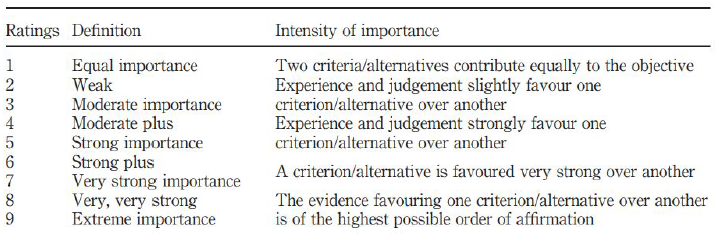
\includegraphics[width=15cm, height=5cm]{figure/auxiliary/fig44.PNG}
    \caption{ Weights to compare importance, used from Shahin(2007)}
    \label{fig:4.4}
\end{figure}
    \item \textbf{Step 5:}
    Selection of KPIs that are more relevant to organizational goal.
    \\
\end{itemize}

Following this process will help making decisions, which provide clear hierarchy and importance levels of the KPIs.

\section{Survey Design and Structure}
In this section ,the theory behind how the survey was designed and structured is discussed. Initially, the steps to conduct a business survey is described. Then the various scales used to measure the responses are mentioned. In the later stages, the analysis methods used to scrutinize the recorded survey data is presented.\\

\textbf{What is a survey?}\\
A survey can be defined as a process of asking questions to respondents to gain information. But as Church et, al (2017, page 4) define survey with the focus on organization development as “A systematic process of data collection designed to quantitatively measure specific aspects of organizational members' experience as they relate to work”.\\

\subsection{Forms of survey}
Mathers et. al (2007) mention in their article that, mostly the surveys take 2 of the forms.\\

\begin{itemize}
    \item \textbf{Cross- sectional surveys:} Surveys that are carried out at a just one point in time are known as a cross-sectional in design. They usually take a descriptive or exploratory form that simply sets out to describe behaviour or attitude. \\


    \item \textbf{Longitudinal surveys:} A longitudinal survey rather than taking a snap-shot, paints a picture of events or attitudes over time.\\


\end{itemize}

For this research due to time constraints and the intent being to collect insights from employees which are etched from their overall experience at Volvo group, cross sectional surveys was employed.\\

\subsection{Methods of data collection in surveys}
Blair et. al (2013) describe the following methods of data collection:
\\

\begin{itemize}
    \item \textbf{Mail survey:} Here a brief letter of request, a detailed cover letter and the questionnaire is sent to the respondents via mail to respond and then send us back. This procedure consumes a lot of time and resources.\\
    
    \item \textbf{Telephone survey:} The selected respondents are dialled and contacted on telephone to discuss the questions and get their answers. This method is applicable when the information to be given by respondents is not easily expressible and the time is feasible.\\

    \item \textbf{Face to face survey:} This is similar to structured interviews. The respondents are questioned based on the list of questionnaire prepared and the answers are recorded.\\

    \item \textbf{Online/Internet survey:} Here the questionnaire along with the introduction, instructions and the intent of survey is sent using the Internet. This method ensures that the speed of data collection is high with the lowest cost possible.\\

\end{itemize}
For this thesis, the Online survey method was chosen using Google forms as the medium. This ensured the data collected to be grouped and analysed easily in the future. Also, it was easily possible to spread the survey to hundreds of intended respondents.\\


\subsection{Stages of survey design}
Church et, al (2017) describe the following 7 step process to design an organizational survey:\\

All the 7 steps are briefly described below:\\

\begin{itemize}
    \item \textbf{Pooling resources:} Church et al (2017) detail this step as, Gaining substantive input and co-operation from all key parties in the organization to get appropriate support to have a survey with good impact.
    \\

    \item \textbf{Designing and developing:} In this step we will look at characteristics of the questions themselves, the content, the response options and scales, the layout or presentation and the formal instructions, to name a few.\\

    \item \textbf{Communicating objectives:} Here the focus is on communicating the purpose, objectives and content of the survey initiative clearly and effectively to those involved in the data collection effort.
\\

    \item \textbf{Administering and improving:} This step includes everything from establishing a clear project plan with appropriate milestones, release the survey and solve the inevitable glitches that occur. Also, based on the preliminary pilot test of the survey, the improvements are done\\

    \item \textbf{Analysis and interpreting:} Interpreting results is one of the most potentially complex and subsequently misunderstood aspects of survey work. It requires the practitioner to identify the main issues and important relationships among a mass of data in what is also often the shortest time frame of the entire survey effort.\\

    \item \textbf{Delivering results:} This step is concerned with the actual delivery of the survey results to organizational members both in various forms and throughout different levels. In ‘Delivering the findings’ the emphasis is on picking a strategy for delivering the feedback to all those involved in the organization.
\\

    \item \textbf{Transferring and action planning:} This step focuses on ‘Learning into action’. The data should be used to drive change and improvements in the system or in people’s day-to-day behaviours. The issues of action planning, identifying areas for intervention and improvement, enlisting and involving others in the process, measuring progress over time through resurvey efforts and linking survey results to other key measures of organizational performance must be performed here.
\\

\end{itemize}
After describing the various stages to deliver an effective organizational survey, the main focus in the next phase is how to design the questionnaire. The considerations to be taken and the different types of scales used are discussed ahead.\\


\subsection{Guidelines for Survey questionnaire}
Questionnaire can be described is the heart of survey research. Structure of survey and the way the questions are presented play an important role in the quality of responses received. Questions can be asked in many different ways, some factual questions to directly comprehend or some opinion based questions which makes the respondents think. Yet, the perception of the survey producer and respondents should match to get effective survey results. Clifford et. al (2016) in their book describe the guidelines to make effective survey questionnaire. They propose three basic principles and five things to avoid.\\

Three basic principles are:\\
\begin{itemize}
    \item \textbf{Keep it simple:} This is to avoid complex phrases and long words that might confuse the respondents.\\
    \item \textbf{Define terms clearly:} Don't assume that respondents are familiar with the terms used. Therefore, define the terms as clear as possible to avoid vague concepts.\\
    \item \textbf{Use simplest possible wording:} So that every respondent irrespective of their command on the language & concept can provide their opinions.\\

\end{itemize}

Five things to avoid:
\begin{itemize}
    \item \textbf{Long complex questions:} These type of questions can confuse the respondents resulting in ineffective responses.\\
    \item \textbf{Two or more questions in one:} The answers received will be too complex which will be tough to analyze further.\\
    \item \textbf{Jargon:} The usage special words or expressions should be avoided as much as possible. If necessity arises, then they should be defined clearly.\\
    \item \textbf{Biased or emotionally charged terms:} These should be reduced to avoid bad responses.\\
    \item \textbf{Negative words:} Usually, the usage of negations tends to confuse the respondents.\\

\end{itemize}

\subsection{Scales used in survey}
Krosnick et. al (1997) mention that, Rating scales are omnipresent in contemporary surveys measuring subjective phenomena such as attitudes and beliefs. Therefore, appropriate development of scales is very important to capture the insights of respondents. In another book on Psychology research, the authors (Fredrick et, al. 2005) proclaim that, It is important to distinguish among the various types of response scales in order to properly code responses and to facilitate the application of statistical analyses.\\

Lets begin with the various types of scales which can be used in surveys as mentioned in Fredrick et. al (2005).\\
\begin{itemize}


\item \textbf{Nominal scales:} Here the variables are categorical in nature. This means that the numerical values assigned to the variables have no real numerical value, but just describe categories. Usually, these are used to measure the factual information such as demographics.\\

\item \textbf{Ordinal scales:} They are used to rank the survey items. One thing to note is, there is a difference between the various choices available, but the magnitude of difference is not indicated. For example, How was the service? The ordinal scales could be Best > Good > Worst.\\

\item \textbf{Interval scales:} The most common interval scale used is the likert scale. It is usually used to measure the satisfaction or dissatisfaction in the opinion oriented surveys. Here the respondents are allowed to choose only one option.\\

\item \textbf{Multiple choice:} This kind of scale is used when there are multiple feasible options a respondent can connect to. Here they have the option to choose one or more options to indicate their preference.\\

\item \textbf{Close ended questions:} These are more specific in nature and easy to interpret. Normally, both the survey creator and respondents perceive these questions in the same way resulting in effective responses.
\\

\item \textbf{Open ended questions:} These questions provide more freedom to the respondents to express their views. These are useful when the knowledge about the concept is not available for survey creators before and they are seeking detailed responses to gain understanding.
 \\
\end{itemize}

Knowledge and proper usage of all these scales accordingly will result in a successful survey questionnaire. But, some considerations must be taken in the usage of these scales.Krosnick et. al (1997) speak about 3 important factors to consider in this regard.\\

\begin{itemize}

\item \textbf{Number of scale points:} When using ordinal or interval scales, the question arises of how many scales should be used. Krosnick et, al (1997) in their research conclude that the scale should be around 5-7 points as it will be more reliable and valid than shorter or longer scales.\\
Also, the usage of even number of scales avoids the possibility of neutral selection.\\

\item \textbf{Labeling the scale points:} The conundrum always arises whether to label all the scale points or only the extreme ones. Krosnick et. al (1997) conclude in their research that, responding to scales with only the endpoints verbally labeled may be less cognitively demanding than scales that are fully labeled. \\

\item \textbf{Inclusion of no-opinion options:} Usually when we probe attitude questions in the survey, we assume that the respondents align to the opinions listed in the survey. But, there might be some cases where the respondent perceives the question in different way and is not clearly inclined or not selecting the clear opinion. Therefore, the opportunity to express his/her views to be neutral or write their thinking in detail should be given.\\
\end{itemize}

\subsection{Kano theory and questionnaire}
All the scales mentioned above can be used to capture the attitudes, insights and facts about the data. But to elicit future needs we need a different method. Sauerwein et. al (1996) describe that using Kano’s model of customer satisfaction,  a methodology can be introduced which determines the influence of the components of products and services have on customer satisfaction. In our case, this idea will be used the capture the customer (PE-employees) needs about KPIs, strategy and performance measurement.\\

Kano theory:\\
    \begin{figure}[H]
    \centering
    \captionsetup{justification=centering, margin=2cm}
    \vspace{1cm}
    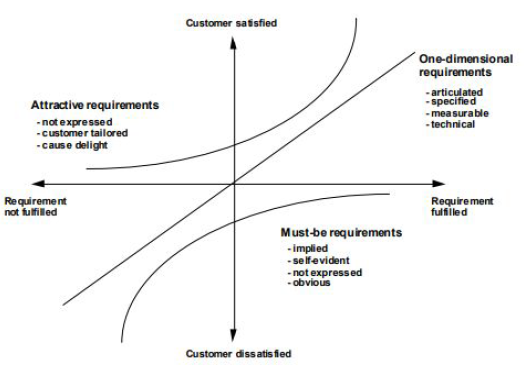
\includegraphics[width=12cm, height=9cm]{figure/auxiliary/fig45.PNG}
    \caption{Kano Model}
    \label{fig:4.5}
\end{figure}\\
As presented in the figure \ref{fig:4.5} and further described by Berger et. al. (1993), Kano model classifies the needs of customers majorly into 3 different aspects.\\

\begin{itemize}
\item \textbf{Must be requirements:} As the name signifies, the customer expects these requirements to be fulfilled, else he will be dissatisfied. On the other hand, it does not increase the satisfaction as the customer takes it to be granted.\\

\item \textbf{One dimensional requirements:} These are explicitly informed by the customer. As visible from the graph above, the customer satisfaction is directly proportional to the requirements fulfilled.\\

\item \textbf{Attractive requirements:} These have a prominent influence on customer satisfaction. These are hard to elicit because they are not stated explicitly by the customer. But, if these are not fulfilled, it will not lead to any dissatisfaction.\\
\end{itemize}

\subsubsection{Construction of Kano Questionnaire}
Using the kano questionnaire, the requirements of customer can be classified into must-be, one dimensional, attractive or indifferent (where customer satisfaction does not matter to requirement). \\

For each product feature a pair of questions is formulated to which the customer can answer in one of five different ways (Kano, 1984). The five different ways are:\\
\begin{itemize}
    \item I like it that way
    \item It must be that way
    \item I am neutral 
    \item I can live with it that way 
    \item I dislike it that way\\
\end{itemize}
First question captures the reaction of the customer if the feature is present and the second question if the feature is not present. Basically, one positive and one negative question is asked about the same requirement. One more point to note is, voice of the customer is the focal point. The "voice of the customer" is a description of the problem to be solved from the customer’s viewpoint” (Sauerwein, 1996) \\

Further steps of the Kano survey is described in the Kano analysis section.\\

\subsubsection{Survey analysis}
In this section, the theory behind the analysis of the data collected during the survey is described.\\

The numerical, quantifiable and demographic data does not need any extensive analysis. As the numerical values/graphs themselves provide the insights to the questions asked. The sections which need analysis are the Kano questionnaire and the open ended questions were coding has to be done.\\

\subsection{Kano analysis}
The answers to two kano questions answered forms the basis for the analysis to conclude the requirement. The figure \ref{fig:4.6} below helps to classify the response of one respondent on both the kano questions into must-be, one dimensional, attractive, indifferent and reversible.\\

For example, if one respondent had chosen ‘Like’ for positive question and ‘must be’ for negative question, then his requirement is classified as “attractive”. Similarly, the responses of each respondent for each requirement is noted down and classified.\\

As mustbe, one dimensional and attractive was explained before. The other 3 aspects are briefly described here:

\begin{itemize}
\item \textbf{Indifferent:} It means that the respondent has no preference in this matter. They are not unsatisfied if absent or satisfied if the measure is present.\\
    \begin{figure}[H]
    \centering
    \captionsetup{justification=centering, margin=2cm}
    \vspace{1cm}
    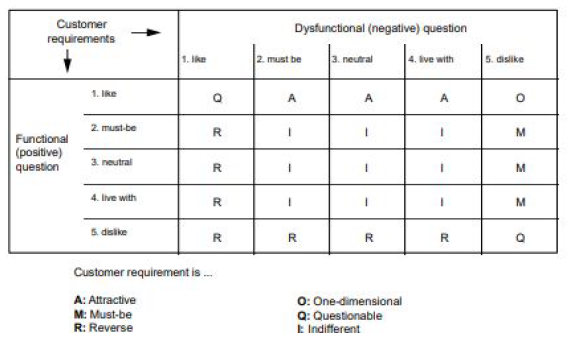
\includegraphics[width=14cm, height=9cm]{figure/auxiliary/fig46.PNG}
    \caption{ Classification of responses for Kano questionnaire}
    \label{fig:4.6}
\end{figure}



\item \textbf{Reverse:} TIt is the opposite of attractive. The fulfilment of attribute will lead to dissatisfaction\\

\item \textbf{Questionable:} This means that the respondent has not understood or unwilling to give a clear preference, but instead has opted for confusing result.\\
\end{itemize}


\subsubsection{Evaluation of kano results}
After the individual responses are noted down, it will be the time to interpret the kano results.\\
As per (Sauerwein, 1996) Majorly it can be done in 3 ways:\\

\begin{itemize}
\item \textbf{Evaluation according to frequencies:} It is one of the easiest methods to analyze the results. It is evaluated based on the frequencies of the answers. Suppose among the 3 requirements asked, the requirement gaining maximum frequency of must-be, one dimensional or attractive are calculated directly. Thus, the nature of each requirement is clear.\\

\item \textbf{Evaluation rule M>O>A>I:} (Must Be, One dimensional, Attractive, Indifferent)
If the individual product requirements cannot be unambiguously assigned to the various categories, the evaluation rule "M>O>A>I" is very useful (Sauerwein, 1996). For example, if all the 3 requirements asked are individual to each other, then this method helps to qualify the importance levels needed. Therefore, the requirements are classified based on the M>O>A>I rule, as it is very important to provide must be requirements as compared to others.\\

\item \textbf{Customer satisfaction coefficient:} Berger et al. (1993) define that, The customer satisfaction coefficient states whether satisfaction can be increased by meeting a product requirement, or whether fulfilling this product requirement merely prevents the customer from being dissatisfied.\\
\end{itemize}
Extent of satisfaction: (A+O) / (A+O+M+I )\\
Extent of dissatisfaction: -(minus) (O+M) / (A+O+M+I)\\

\subsection{Coding}
In this section, the various academic theories behind coding is discussed. The previous section on coding focussed only on qualitative interviews. Whereas, this part discusses in detail starting from definition of coding, approaches to creation of codes, different types of coding and the content analysis which is the focal part of the survey.\\

Coding is one of the important steps in qualitative research. Ely et al. (1991) opine that we come to qualitative research with whatever understanding of analysis we bring from previous work, the conventions of our respective disciplines and professions, the advice of our mentors and the models we have internalized from whatever we have read. But to effectively transfer our internal tacit knowledge for other people, a definitive method is needed to categorise our findings. Here is where the codes come into picture.Basit (2003) describes that this process of coding is dynamic, intuitive and creative process of inductive reasoning, thinking and theorizing.\\

\subsubsection{Definition of coding}
Saldana (2015, page 4) defines that “A code in qualitative inquiry is most often a word or a short phrase that symbolically assigns a summative, salient, essence capturing and evocative attribute for a portion of language-based or visual data.” 


\subsubsection{Approach to creation of codes}
Miles and Huberman (1994) mention two approaches to create the codes. \\
\begin{itemize}
    \item The first one is used by the inductive researcher, where there are pre-codes created. This is in conjunction to the grounded theory approach mentioned by Glaser and Strauss. The codes are thought of only after thee data is collected and variety of codes are designed.\\
    \item The second approach is to create a initial start list of codes before the empirical data is collected. These initial codes come from the research questions, hypothesis or the key variables of the study undertaken. \\
\end{itemize}
In this study as we are using the approach with inductive thinking, the codes which come under this are discussed.\\

\subsubsection{Types of coding}
The two types of coding under the grounded theory study are substantive coding and theoretical coding.\\

\begin{itemize}
    \item \textbf{Substantive coding:} Here the researcher works with the data directly, fracturing and analyzing it, initially through open coding for emergence of code category and subsequently through selective coding to theoretically saturate the core and related concepts. This type of coding is used mostly in our study here.\\
    \item \textbf{Theoretical coding:} This is achieved by constantly comparing the indicators in the data to elicit the properties and dimensions of each category. (Bryant & Charmaz, 2007, page 265)\\
\end{itemize}

These 2 types of coding types help to effectively use the academic research in this study and employ the correct approach before start of coding.\\

\subsubsection{Content analysis}
To analyse the various open ended questions in our survey, the understanding is needed how to look through the content available and then come to conclusions. In their article on qualitative content analysis, Hsieh & Shannon (2005) discuss three different approaches:\\

\begin{itemize}
    \item \textbf{Conventional:} Here the coding categories are directly defined from the collected empirical \\
    \item \textbf{Directed:} In this case, the analysis begins with theory as a guiding factor to generate initial codes\\
    \item \textbf{Summative:} A summative content analysis involves counting and comparisons, usually of keywords or content, followed by the interpretation of the underlying context.\\
\end{itemize}
As far as the survey analysis is concerned, conventional approach to content analysis was employed most of the times. Only once or twice for specific survey questions summative approach was used.\\




